
\section{John Backus}

IBM did not feel that Aiken and the Harvard Computation Laboratory had given
them sufficient credit for their contributions to the Mark I, which left
Thomas Watson Sr. and the IBM folks bitter about the experience and eager to
produce a new device entirely in-house. This device would become the Selective
Sequence Electronic Calculator, or the SSEC. It was built on 57th Street in
Manhattan, and it was monstrous. Roughly 50 by 100 feet with a giant console
and hundreds of toggle switches and tape units and relays behind glass panels;
there were giant windows that allowed passersby to see the machine in action.

One such passerby was John Backus, a recent Masters graduate from Columbia
University. He was intrigued by the machine, which he mentioned to his tour
guide, who suggested he go upstairs and talk to the boss about it. Robert "Rex"
Seeber gave him a puzzle, which he solved, and he was hired on the spot
\cite{backus_oral_history_2006}.

In 1942, Backus majored in Chemistry at the University of Virginia where he
struggled academically. He was expelled due to poor attendance within the first
year before being drafted into the US Army. He commanded an antiaircraft
battery at Fort Steward, Georgia, remaining in the US for the remainder of
WWII.

While he did not at first find success in academia, he got very good marks on
military aptitude tests. He was directed to the University of Pittsburgh's
engineering program and later to a premedical program at Haverford College near
Philadelphia (which is where he grew up). In 1945 he attended the Flower and
Fifth Avenue Medical School in NYC, but he was still struggling with the
academy. He was uninterested in medicine, feeling that it was all about
memorization. He dropped out after less than a year.

He entered a radio technician school and became interested in math, which led
him to enroll in the math program at Columbia University. The SSEC that would
intrigue him at the IBM computing center was designed at the Watson Scientific
Computing Laboratory at Columbia.

\section{IBM Mathematical FORmula TRANslating System}

At IBM, Backus worked on the SSEC and later the IBM 701 and 704. The main use
of the SSEC was aerospace calculations; programming calculations to predict the
position of the moon was one of the first tasks he was given at IBM. He would
continue writing programs for these machines in spite of their poor usability.
His team's techniques would be used in the lunar missions of the 1960s.

The pain of writing programs for these early machines entirely in machine code
drove him to explore new ways to program. The first of these was a symbolic
notation for floating point arithmetic and address expression calculation
called Speedcoding\cite{backus_oral_history_2006}:

\begin{quotation}
  \textbf{Grady Booch:}
  So then from your experience with the SSEC, you then went on to
  produce Speedcoding, the
  Speedcoder\dots
  What were sort of the things that influenced you to create that in
  the first place?

  \textbf{John Backus:}
  Well, programming in machine code was a pretty lousy business to
  engage in, trying to figure
  out how to do stuff. I mean, all that was available was a sort of a
  very crude assembly program. So I
  figured, well, let's make it a little easier. I mean it was a
  rotten design, if I may say so, but it was better
  than coding in machine language.
\end{quotation}

The IBM 701 did not have an index register, so calculating addresses for array
operations was tedious and error-prone. Speedcoding provided a way to express
these calculations symbolically.

\begin{figure}[h!]
  \centering
  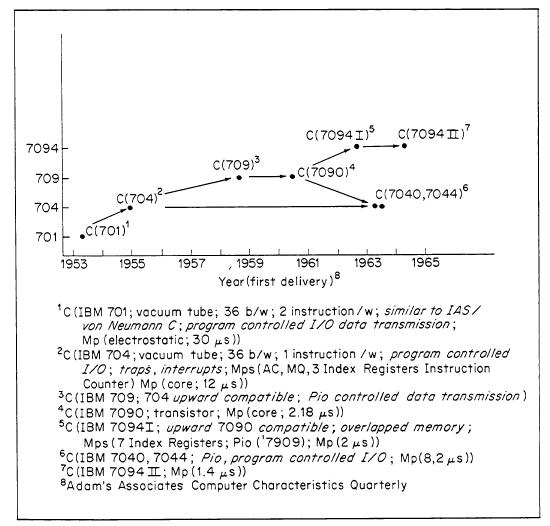
\includegraphics[width=0.5\linewidth]{resource/ibm-7094.jpeg}
  \caption{Excerpt from \textit{The IBM 701--7094 II Sequence: A
    Family by Evolution}
    \cite{Hamming_Feigenbaum_1971_IBM7094}, illustrating the
  instruction structure for summing quantities.}
  \label{fig:ibm7094-example}
\end{figure}

The 704 was the first machine to have such a register; it also had floating
point instructions and core memory, more or less obviating the need for
Speedcoding: "we were moving to the 704, which had built in floating point,
built in index registers, which was all that Speedcoding was supposed to
supply. So what the hell?" \cite{backus_oral_history_2006} He credits himself
with getting index registers and floating point into the 704.

%Here is an example from the IBM Speedcode manual\cite{IBM_1954_Speedcoding}:
%\begin{quotation}
%    Assume that it is necessary to compute the sum of 34 quantities stored in
%    locations 688 through 721 and to store the sum in cell 945.
% Assume further that
%    cell 1013 contains the number zero and that instruction 416 is the next
%    instruction to be executed. The sequence of instructions shown
% below could be
%    used for this purpose:
%
%    \begin{center}
%    \begin{tabular}{cccccccc}
%    \hline
%    LOC & OP$_1$ & R & A & B & C & OP$_2$ & D \\
%    \hline
%    0416 & ADD  & 0 & 1013 & 1013 & 0945 & SETRA & 0000 \\
%    0417 & ADD  & 4 & 0688 & 0945 & 0945 & SKRA  & 0033 \\
%    0418 & NOOP & 0 & 0000 & 0000 & 0000 & TIA   & 0417 \\
%    \hline
%    \end{tabular}
%    \end{center}
%\end{quotation}

\begin{figure}[h!]
  \centering
  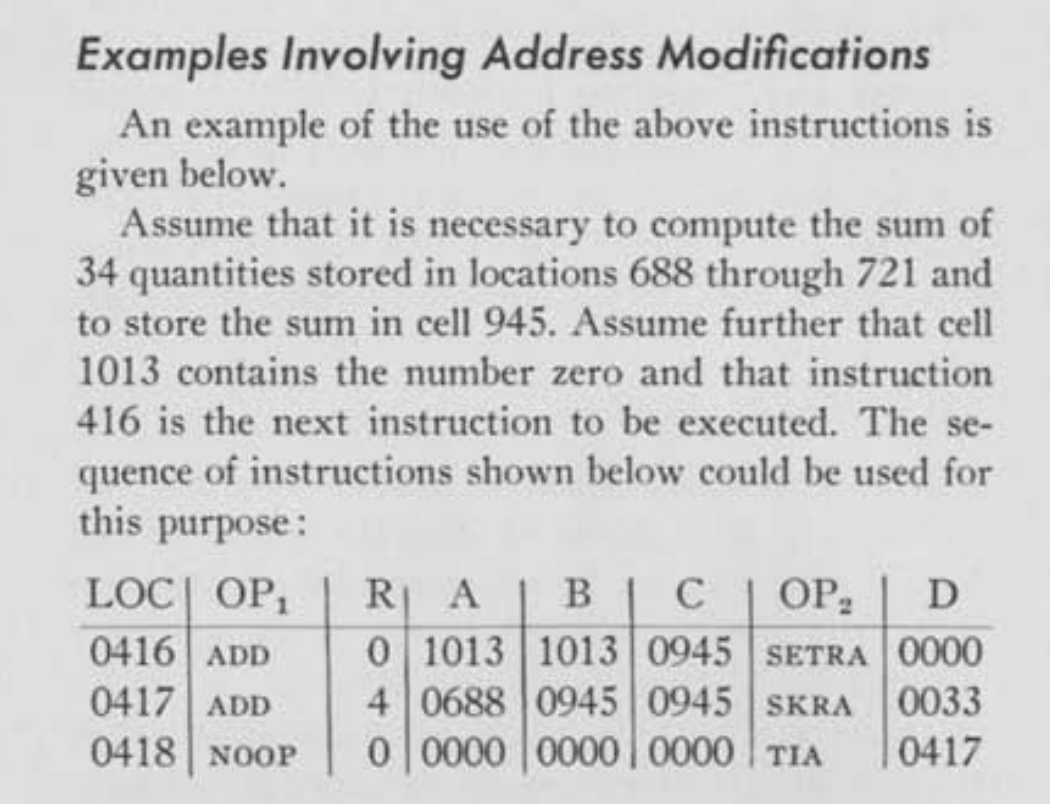
\includegraphics[width=0.5\linewidth]{resource/ibm-speedcoding-example.png}
  \caption{Excerpt from \textit{IBM Speedcoding for the Type 701
    Electronic Data Processing Machine}
  \cite{IBM_1954_Speedcoding}}
  \label{fig:ibm-speedcoding-example}
\end{figure}

Backus did not think all that highly of Speedcoding in retrospect, though it
gained traction in large part due to IBM's marketing power and the number of
users of the 701 relative to the size of the computer market at the time
\cite{Backus_1980_Programming_in_America_in_1950s}. It is unclear whether
Backus's assessment of his own code is accurate or if it's born of humility.

\begin{quotation}
  The success of some programming systems depended on the number of machines
  they would run on. Thus, an elegant system for a one-of-a-kind machine might
  remain obscure while a less-than-elegant one for a production
  computer achieved
  popularity. This point is illustrated by two papers at the 1954 ONR symposium
  One, by David E. Muller, describes a floating point interpretive system for
  the ILLIAC designed by D. J. Wheeler. The other, by Harlan Herrick and myself,
  describes a similar kind of system for the IBM 701 called Speedcoding. Even
  today Wheeler's 1954 design looks spare, elegant, and powerful, whereas the
  design of Speedcoding now appears to be a curious jumble of compromises.
  Nevertheless, Wheeler's elegant system remained relatively obscure (since only
  ILLIAC users could use it) while Speedcoding provided enough conveniences,
  however clumsily, to achieve rather widespread use in many of the eighteen 701
  installations.
\end{quotation}

In 1953, based on his experience with Speedcoding on the 701, Backus proposed
yet another language to elevate the programming experience on the 704. IBM
management supported the proposal. He formed a ten-person team of his own
choosing based out of IBM's Manhattan headquarters, including Irving Ziller,
\todo{list other members}. They released \textit{Preliminary Report,
  Specifications for the IBM Mathematical FORmula TRANslating System,
FORTRAN}\cite{IBM_1954_FORTRAN_Specifications} after about one year of working
together. Roughly two years after its first conception, \FTN{} was released for
the first time. It would go on to ship with every IBM 704 and become the
primary means of programming in the scientific community. Backus could not
stand how slow programming was without a higher-level language, and machines
were expensive; leasing a machine and spending time programming in machine code
wasted money compared to a compiler capable of generating reasonable machine
code (though at the time it usually underperformed hand-written code). Backus
and his team would continue to develop and stabilize this compiler for several
years, though.

\begin{quotation}
  \FTN{} did not really grow out of some brainstorm about the beauty of
  programming in mathematical notation; instead it began with the recognition
  of a basic problem of economics: programming and debugging costs already
  exceeded the cost of running a program, and as computers became faster
  and cheaper this imbalance would become more and more intolerable. This
  prosaic economic insight, plus experience with the drudgery of coding, plus
  an unusually lazy nature led to my continuing interest in making
  programming easier.
  This interest led directly to work on Speedcoding for the 701
  and to efforts to have floating point as well as indexing built into the 704.
  \cite{Backus_1980_Programming_in_America_in_1950s}
\end{quotation}

When Backus was forming his team in January of 1954, he was moved from the Pure
Science department at IBM into the Applied Science department because his boss
Rex Seeber wanted nothing to do with the project. There he found Irving Ziller,
who became his first teammate. By April, they had been joined by Harlan Herrick
who co-authored the Speedcoding paper with Backus at the ONR symposium
\citetitle{Backus_Herrick_1954_Speedcoding} in which they observe:

\begin{quotation}
  The question is, can a machine translate a sufficiently rich mathematical
  language into a sufficiently economical program at a sufficiently low cost to
  make the whole affair feasible?  consider the advantages of being
  able to state
  the calculations\dots for a problem solution in a concise, fairly natural
  mathematical language.
\end{quotation}

The reader should note that it is often incorrectly asserted (at times even by
Backus himself\cite{Backus_1980_Programming_in_America_in_1950s}) that this
came \textit{after} Backus and Ziller had been given a demonstration of Laning
and Zierler's algebraic compiler for the Whirlwind at MIT at the ONR symposium
of 1954. When they received this demonstration, there were already four members
of the \FTN{} team, Irving Ziller, Robert Nelson, Harlan Herrick, and Backus
himself. In Backus's words\cite{Backus_1980_Programming_in_America_in_1950s}:

\begin{quotation}
  The article and the letter therefore show that, much to my surprise, the
  FORTRAN effort was well under way before the ONR symposium and that,
  independently of Laning (but later), we had already formulated more ambitious
  plans for algebraic notation (e.g., Gail bjk) than we were later to find in
  Laning and Zierler's report and see demonstrated at MIT. It is therefore
  unclear what we learned from seeing their pioneering work, despite my mistaken
  assumption over the years that we had gotten our basic ideas from them
\end{quotation}

Indeed, even Grace Hopper at a 1956 symposium made the same assertion:

\begin{quotation}
  A description of Laming and Zierler' s system of algebraic pseudocoding for
  the Whirlwind computer led to the development of Boeing 's BACAIC for the 701,
  FORTRAN for the 704, AT-3 for the Univac, and the Purdue System for the Datotron and. indicated the need for far more effort in the area of algebraic
  translators.
  \cite{Knuth_TrabbPardo_1976_Early_Development}
\end{quotation}

I am not sure who to believe either!

With the support of his new boss Cuthbert Hurd, his family, friends, and his
team, the first report of \FTN{} was released externally to 704 users. This
brought interest from a variety of users, many of whom offered up members of
their teams to help.

\section{\FTN{} Optimization and the First Users}

Setting aside the members of the "priesthood" of computing who were hostile to
the idea of compilers and making programming more accessible, the external
report on \FTN{} brought these contributors into the fold:
\begin{itemize}
  \item Walter Ramshaw at United Aircraft allowed Roy Nutt to work
    with the team; he
    eventually designed and implemented parts of the runtime and I/O features.
  \item Charles W. Adams allowed Sheldon Best to join the team on
    leave from MIT.
  \item Sidney Fernback at the Livermore Radiation Laboratory loaned
    out Bob Hughes.
  \item Harry Cantrell at G.E. was enthusiastic about the project.
\end{itemize}

The team was composed of the following 9 members: David Sayre, Harlan Herrick,
John Backus, Lois Haibt, Robert Nelson, Roy Nutt, Sheldon Best, Richard
Goldberg, and Peter Sheridan.

Most of the skepticism about \FTN{} came from the "priesthood," Backus's
facetious term for the "elite" programmers who thought programming needn't be
made accessible and compilers would never achieve the performance their of
hand-written code. This made the optimization of \FTN{} programs a high
priority for the team; to achieve the widest possible adoption, they would need
to convince even the skeptics that \FTN{} programs could be efficient. In
Backus's 1976 retrospective on programming in the
1950s\cite{Backus_1980_Programming_in_America_in_1950s}, he highlights the
optimization efforts of three members of the original team:

\begin{itemize}
  \item Nelson and Ziller optimized array indexing expressions and
    loop analyses.
    Backus specifies that they could "could move computations from the object
    program to the compiler" which appears to be the first instance of
    constant-folding in a compiler.
  \item Best optimized the use of index registers based on the
    expected hotness of the
    execution path. "As of 1970 there were no known provably optimal
    algorithms for
    the problem he dealt with; his methods were the basis of many subsequent
    storage-allocation algorithms and produced code that is very difficult to
    improve. (For more details of Best's methods see [4, pp. 510-5151.)"
\end{itemize}

This is, as far as I can tell, the first concerted effort to produce an
optimizing compiler.

\section{Language Specification and Backus-Naur Form}

\todo{explain BNF and lang specs, tie in with GH algol
work}\cite{Backus_1980_Programming_in_America_in_1950s}:
\begin{quotation}
The notation for syntax description known as BNF offers another example of a
development which began with a prosaic recognition of a need.
After involvement
with two language design efforts-FORTRAN and IAL (ALGOL 58)-it
became clear, as
I was trying to describe IAL in 1959, that difficulties were
occurring due to
the absence of precise language definitions. In a recent course on
computability given by Martin Davis, I had been exposed to the work of the
logician Emil Post and his notion of a "production." As soon as the need for
precise description was noted, it became obvious that Post's
productions were
well suited for that purpose. I hastily adapted them for use in
describing the
syntax of IAL. The resulting paper [5] was received with a
silence that made it
seem that precise syntax description was an idea whose time had
not yet come.
As far as I know that paper had only one reader, Peter Naur. Fortunately, he
had independently recognized the need for precision; he improved
the notation
(replacing oi: by I and := by : =), improved its readability by not
abbreviating the names of metavariables, and then used it to describe the
syntax of ALGOL 60 in the definitive paper on that language. He
thus proved the
usefulness of the idea in a widely read paper I and it was accepted.
\end{quotation}
% \begin{figure}[h!]
%     \centering
%     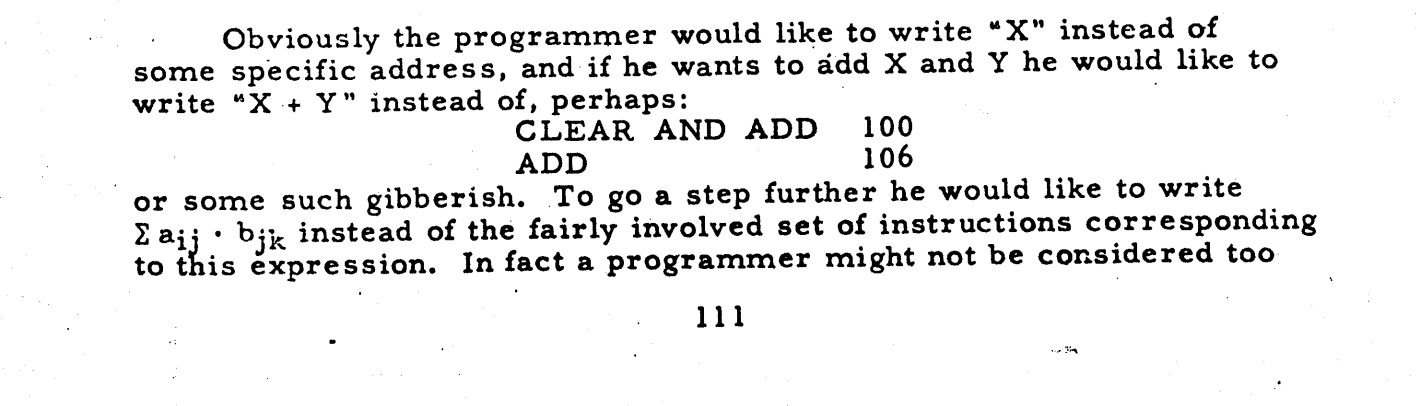
\includegraphics[width=0.5\linewidth]{resource/Backus_Herrick_Speedcoding_ONR_1954.png}
%     \caption{Excerpt from \citetitle{Backus_Herrick_1954_Speedcoding}}
%     \label{fig:backus-herrick-speedcoding-onr-1954}
% \end{figure}

\todo{Backus wasn't really that involved in fortran II and III and IV.
The rest of the team took over. He never wrote much fortran and
doesn't have many thoughts
about it today other that the "we should be making things higher level."}
\todo{Backus moved into functional programming. Was never fruitful.
He became a lab fellow at IBM after Watson Jr started the
fellowship program,
so he could kinda play with functional programming and not really
get much done.}
\todo{He didn't like Hopper's ideas for COBOL, thought they were
crazy and too complex.
Didn't like algol either. Really just wanted to make things
simpler and higher level
and easier to use. Pushed back against the priesthood.}
\todo{the priesthood didn't like fortran because it made things easy.
Backus resisted this urge at every point in his career.
Like GH, he wanted programming to be easy and accessible
(tho he didn't like her direction)}

\begin{quotation}
Though the FORTRAN operator's manual was completed by the fall of 1956, the
compiler itself was not distributed to IBM 704 installations
until April 1957.
Within a year after distribution, half of the IBM 704
installations were using
FORTRAN to solve more than half of all mathematical prob-lems.16
Subsequently,
compilers were produced for the IBM 705 and the IBM 650, quickly
making FORTRAN
the most widely used automatic program of its day. By 1961, UNIVAC users
demanded a compatible FORTRAN compiler and abandoned Hopper's MATH-MATIC.
\cite{grace_hopper_and_the_invention_of_the_information_age_2009}
\end{quotation}

\begin{quotation}
It describes the system which will be made available during late
1956, and is
intended to permit planning and fortran coding in advance of that
time [p. 1],
Object programs produced by fortran will be nearly as efficient as those
written by good programmers [p. 2], "Late 1956" was, of course, a
euphemism for
April 1957. Here is how Saul Rosen described fortran's debut [RO
64, p. 4]: Like
most of the early hardware and software systems, fortran was late
in delivery,
and didn't really work when it was delivered.
\cite{history_of_computing_in_the_twentieth_century_1980}
\end{quotation}

\begin{quotation}
It is not my intention to give a complete description of either; hence this
section will describe only the main highlights of FORTRAN development. The
earliest significant document that seems to exist 1s one marked
"PRELIMINARY REPORT, Specifications for the IBM Mathematical FORmula
TRANslating System, FORTRAN", dated November 10, 1954 and issued by the
Programming Research Group, Applied Science Division, of IBM.
\cite{sammet_programming_languages_history_and_fundamentals_1969}
\end{quotation}

\begin{quotation}
Laning and Zierler's algebraic compiler served as evidence that prestigious
institutions such as MIT were taking automatic programming
seriously, prompting
Backus to write Laning a letter shortly after the May symposium.
In the letter,
Backus informed Laning that his team at IBM was working on a
similar compiler,
but that they had not yet done any programming or even any
detailed planning.12
To help formulate the specifications for their proposed language, Backus
requested a demonstration of the algebraic compiler, which he and Ziller
received in the summer of 1954. Much to their dismay, the two
experienced firsthand the efficiency dilemma of compiler-based
language design. The MIT
source code was commendable, but the compiler slowed down the Whirlwind
computer by a factor of 10. Since computer time was so dear a
commodity, Backus
realized that only a compiler that maximized efficiency could
hope to compete
with human programmers. Despite this initial disappointment, Laning and
Zierler's work inspired Backus to attempt to build a compiler that could
translate a rich mathematical language into a sufficiently
economical program
at a relatively low cost.13
\cite{grace_hopper_and_the_invention_of_the_information_age_2009}
\end{quotation}
